\chapter{Profiling Benchmark Applications} \label{hdrnn-profile}

Flame graphs capturing application performance during a single epoch are listed in the following section. These graphs were formed using the data obtained by the \texttt{perf} profiling utility program. \texttt{perf} was used to collect stack trace information and then this data was used to produce the flame graphs. Flame graphs are an efficient means of representing a large amount of stack trace information. The horizontal axis shows the stack profile for the different stacks that occupy the CPU during the program's execution. The vertical axis shows the stack depth, counting from zero at the bottom. Each rectangle in the graph represents a stack frame. The wider a frame is, the more often it was present in the sampling of the stack traces. The top edge shows what is on CPU and beneath it is its adjacent frames.

\subsection*{Flame graphs from perf Measurements}

\begin{figure}[H]
	\centering
	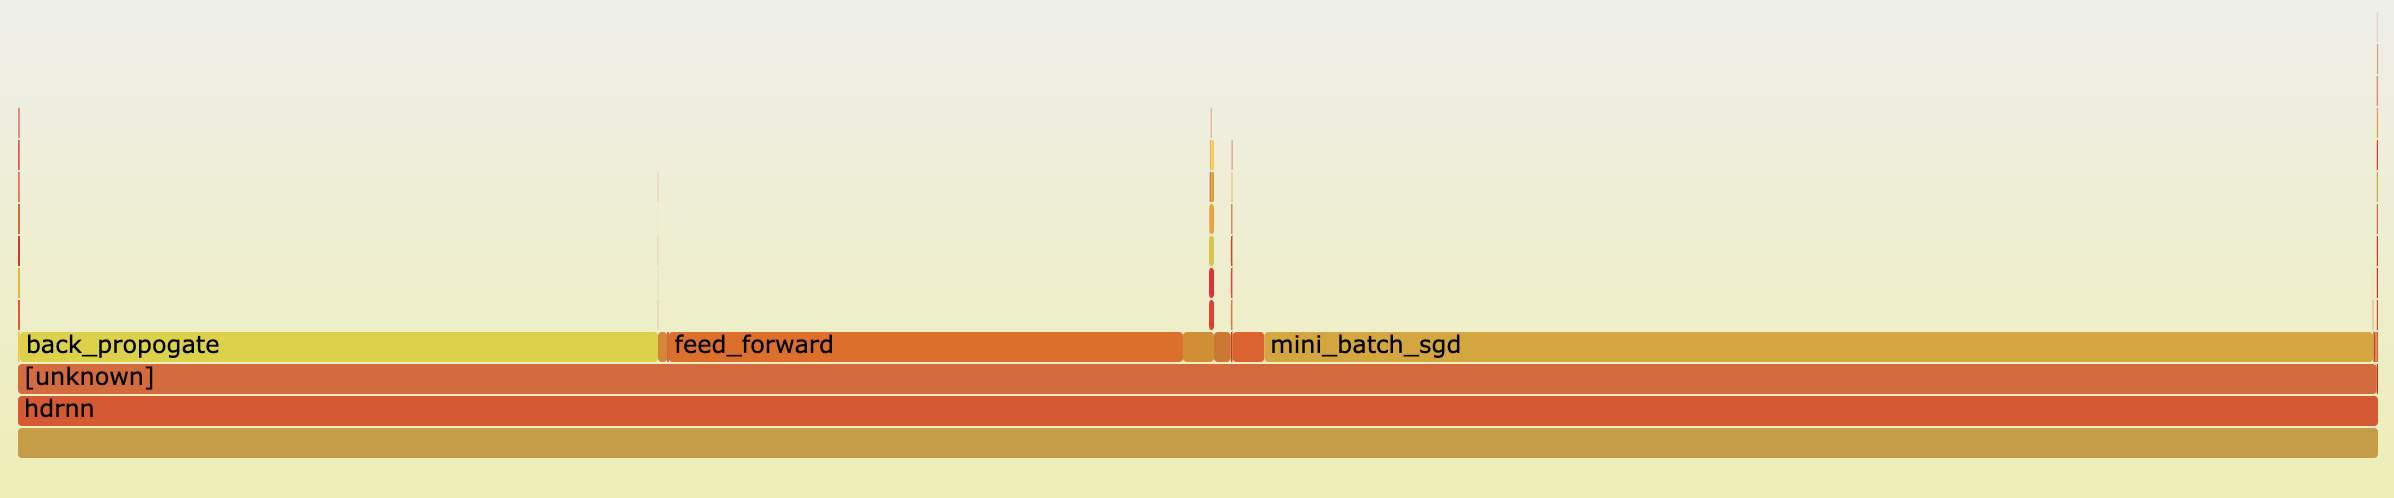
\includegraphics[scale=0.34]{c-math.h-fg.png}
	\caption{c-math.h}
\end{figure}

\begin{figure}[H]
	\centering
	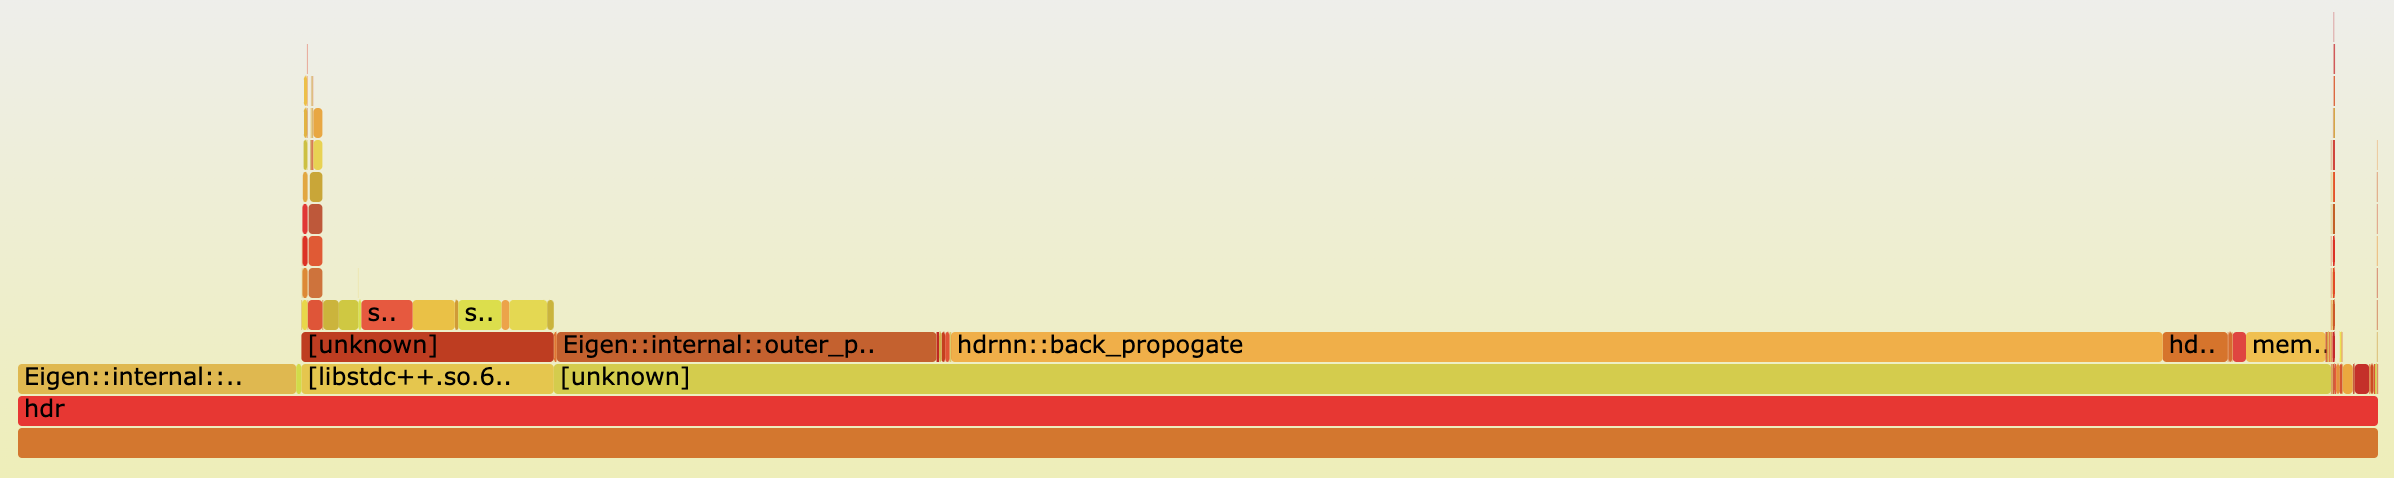
\includegraphics[scale=0.34]{cpp-eigen-fg.png}
	\caption{cpp-eigen}
\end{figure}

\begin{figure}[H]
	\centering
	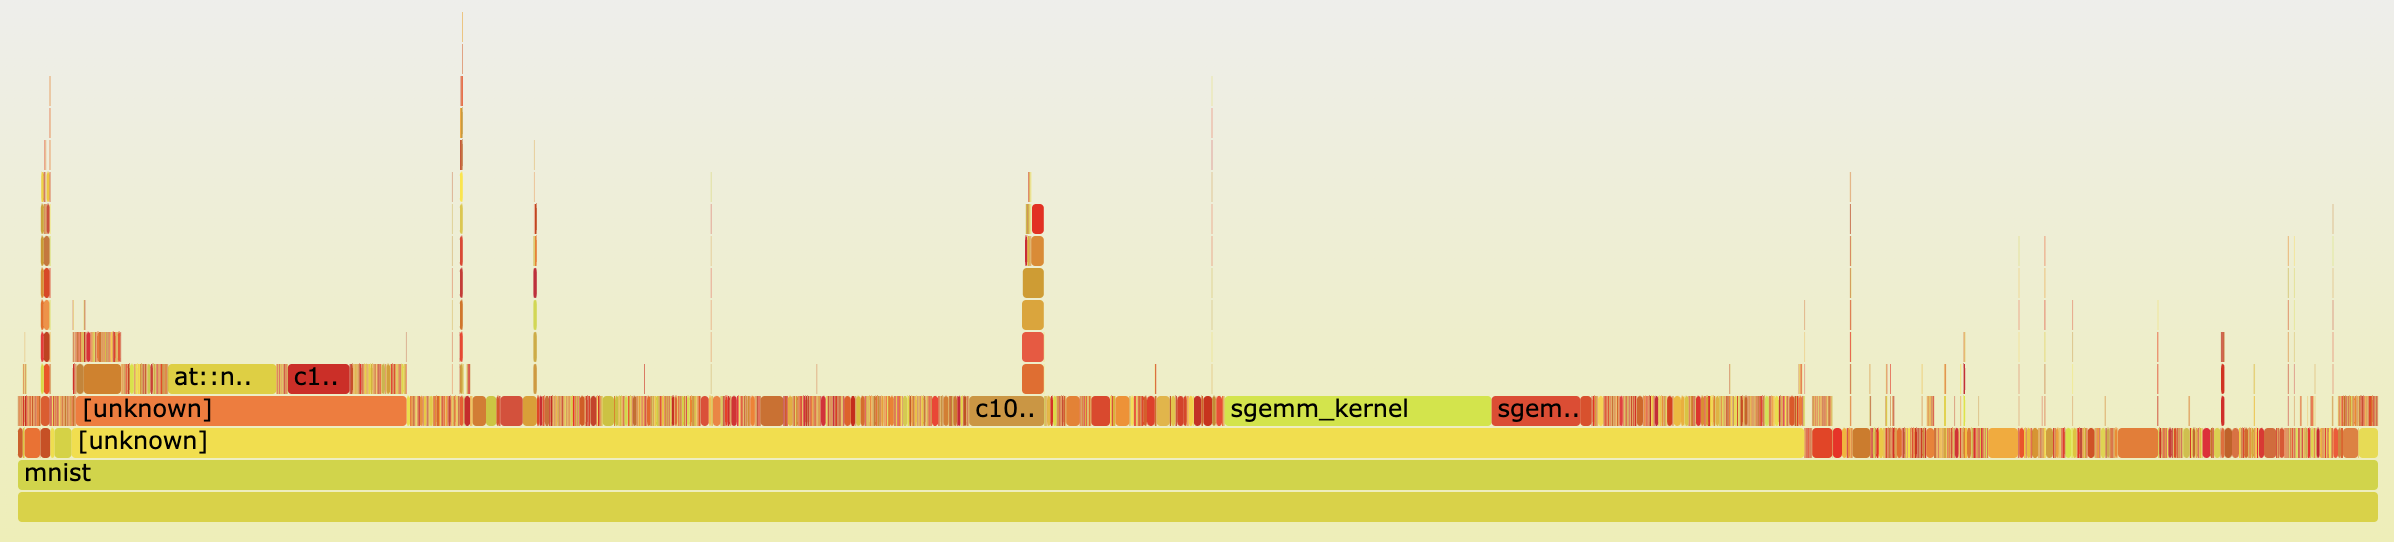
\includegraphics[scale=0.34]{cpp-libtorch-fg.png}
	\caption{cpp-libtorch}
\end{figure}

\begin{figure}[H]
	\centering
	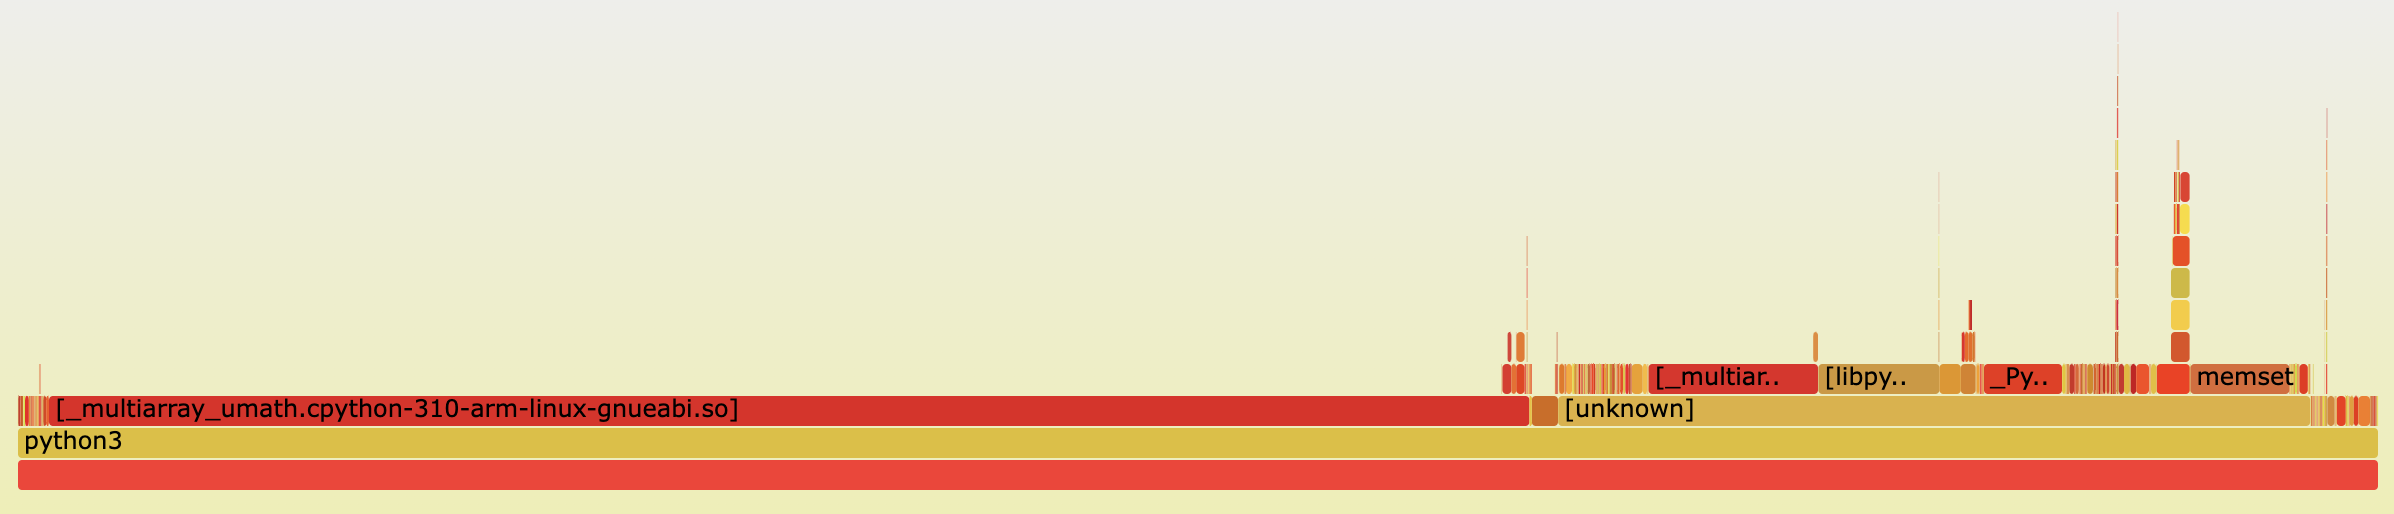
\includegraphics[scale=0.34]{python-numpy-fg.png}
	\caption{python-numpy}
\end{figure}

\subsection*{Memory Profile through Heaptrack} \label{hdrnn-memory-profile}

Heaptrack measurement for C based implementation of HDR-NN running for 4 epochs under different sizes are presented below

\begin{figure}[ht]
	\centering
	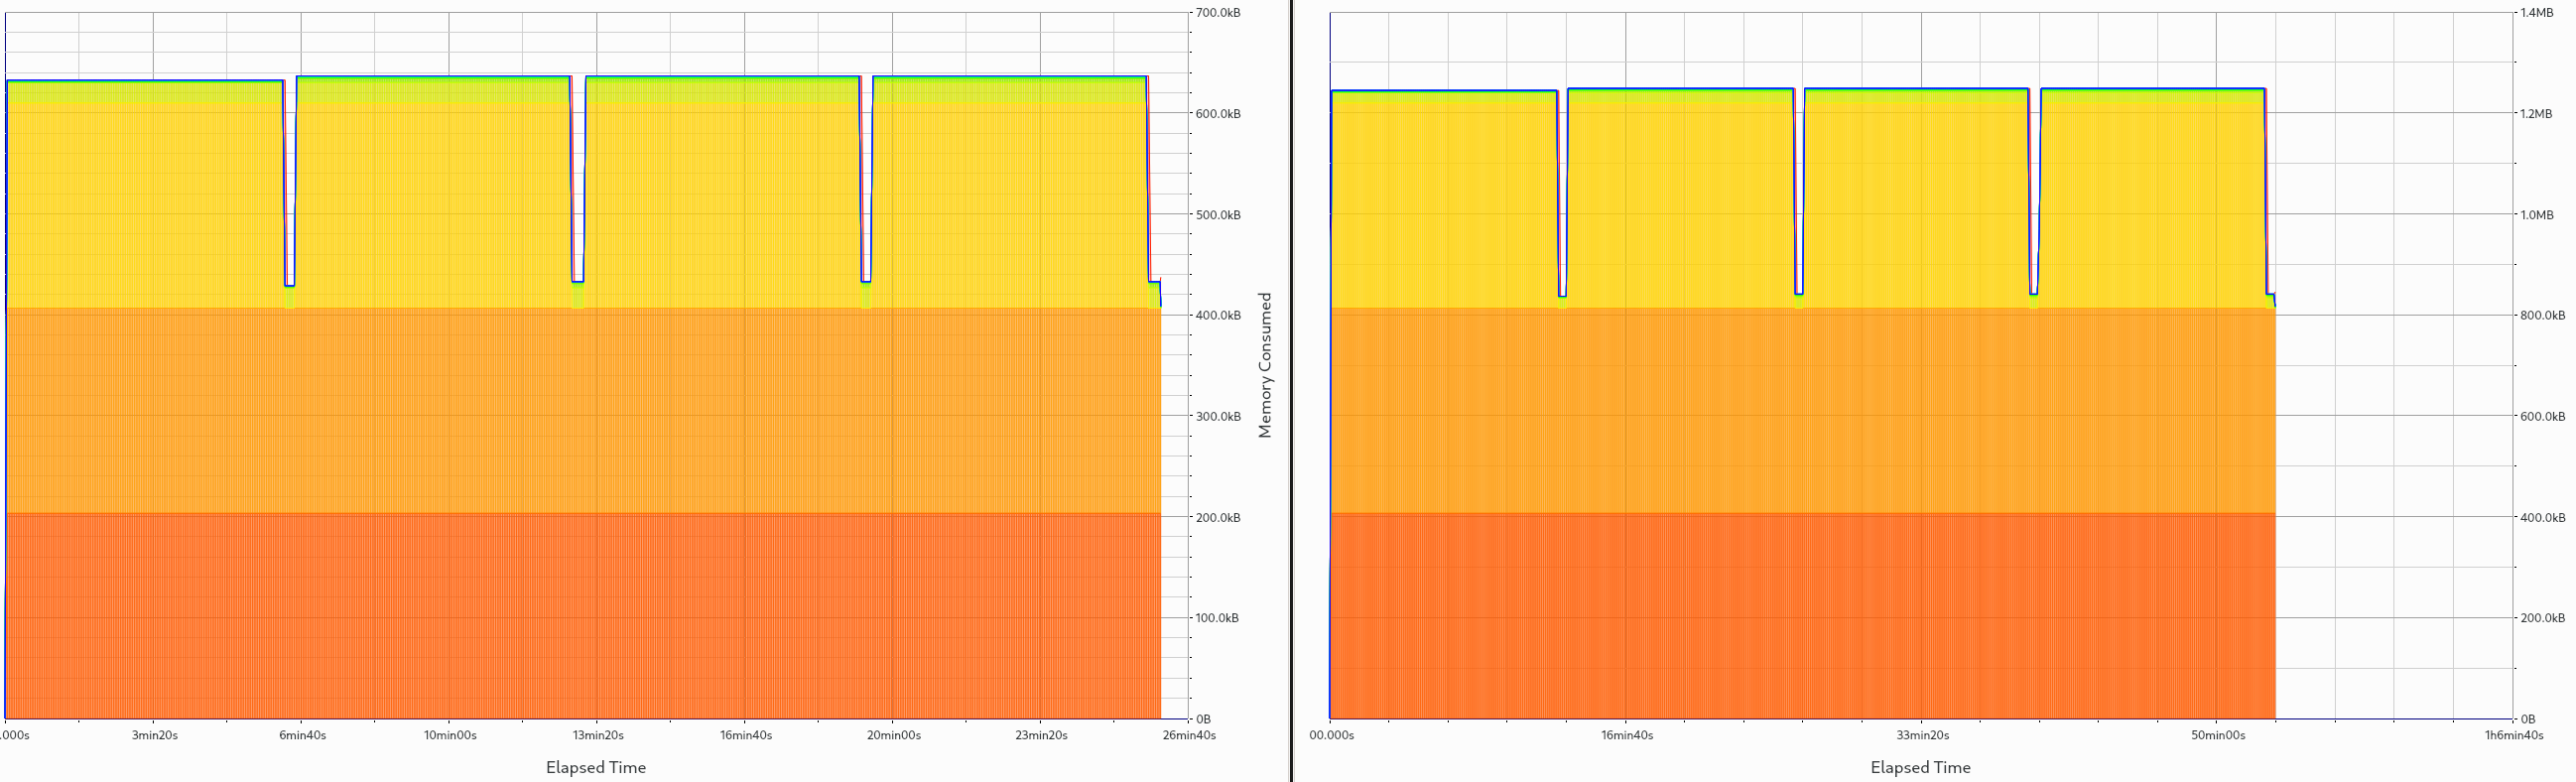
\includegraphics[scale=0.15]{heaptrack-compare.png}
	\caption{\texttt{c-math.h} with different shapes. Plot on the left is for shape 8 while the right is for shape 16.}
	\label{fig:memory-shape}
\end{figure}

The memory allocations of different size as tracked by Heaptrack for a single epoch execution run of the \texttt{c-math.h} implementation for shape 8 is given below.

\begin{figure}[ht]
	\centering
	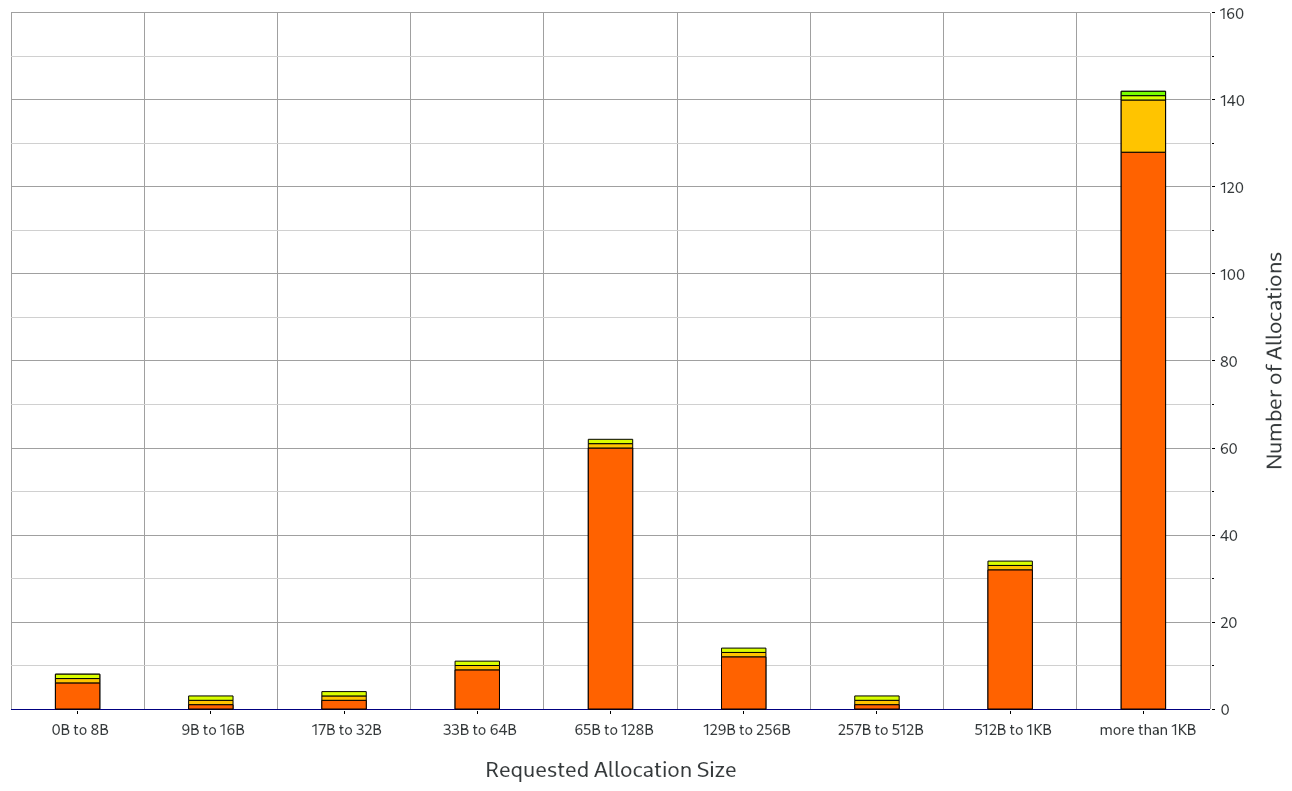
\includegraphics[scale=0.32]{c-math.h-allocations.png}
	\caption{\texttt{c-math.h} allocations}
\end{figure}
